\chapter{Конструкторский раздел}

В данном разделе представлены схемы алгоритмов умножений матриц и их модификации.

\section{Трудоемкость алгоритмов}\label{estimate}
Для получения функции трудоемкости алгоритма необходимо ввести модель оценки трудоемкости. Трудоемкость "элементарных" операций оценивается следующим образом.
\begin{enumerate}
	\item Трудоемкость 1 имеют операции:
	\begin{equation*}\label{math:simple}
		\begin{array}{cc}
			+, -, =, <, >, <=, >=, ==, +=, -=,\\
			++, --, [], \&\&, ||, >>, << \\
		\end{array}
	\end{equation*}
	\item Трудоемкость 2 имеют операции:
	\begin{equation*}\label{math:complex}
		*, /, \char`\\ , \%
	\end{equation*}	
	\item Трудоемкость конструкции ветвления определяется как
	\begin{equation}\label{math:if}
		f_{if} = f_{\text{условие}} + 
		\begin{sqcases}
			min\left(f_{\text{истина}} , f_{\text{ложь}}\right) \text{ в лучшем случае,} \\
			max\left(f_{\text{истина}} , f_{\text{ложь}}\right) \text{ в худшем случае.} \\
		\end{sqcases}
	\end{equation}
	\item Трудоемкость цикла расчитывается как
	\begin{equation}\label{math:loop}
		f_{\text{цикл}} = f_{\text{инициал.}} + f_{\text{сравн.}} + N \left(f_{\text{тело}} + f_{\text{инкремент}} + f_{\text{сравн.}}\right)
	\end{equation}
	\item Трудоемкость вызова функции равна 0.
\end{enumerate}


\subsection{Классический алгоритм}

Пусть на вход алгоритму поступают матрицы $M_{left}$ и $M_{right}$ с размерностью $n \times m$ и $m \times q$. Тогда трудоемкость классического алгоритма равна

\begin{equation}\label{math:alg}
	f_{alg} = 2 + n\left(2 + f_{цикл_j}\right) \approx 14mnq = 14MNQ
\end{equation}
\subsection{Алгоритм Винограда}

Трудоёмкость алгоритма Винограда состоит из следующих этапов:
\begin{itemize}
	\item создания и инициализации массивов MH и MV, трудоёмкость которого равна
	\begin{equation}
		\label{for:init}
		f_{инициализация} = M + N;
	\end{equation}
	
	\item заполнения массива MH, трудоёмкость заполнения  равна
	\begin{equation}
		\label{for:MH}
		f_{MH} = \frac{19}{2}MN +6M +2;
	\end{equation}
	
	\item заполнения массива MV, трудоёмкость заполнения которого равна
	\begin{equation}
		\label{for:MV}
		f_{MV} = \frac{19}{2}QN +6Q +2);
	\end{equation}
	
	\item цикла заполнения матрицы для чётного N, его трудоёмкость равна
	\begin{equation}
		\label{for:cycle}
		f_{\text{цикл}} = 16MQN + 13MQ + 4M + 2;
	\end{equation}
	
	\item цикла для дополнения умножения суммой последних элементов перемножаемых строки и столбца, если линейная размерность N нечётная, трудоемкость этого цикла равна
	\begin{equation}
		\label{for:last}
		f_{\text{последний}} = 3 + \begin{cases}
			0, & \text{чётная,}\\
			16MQ + 4M + 2, & \text{иначе.}
		\end{cases}
	\end{equation}
\end{itemize}

Итого, для худшего случая (нечётный размер матриц N) трудоемкость равна
\begin{equation}
	\label{for:bad}
	f =  f_{MH} + f_{MV} + f_{cycle} + f_{last}\approx 16 \cdot MNQ
\end{equation}

Для лучшего случая (чётный размер матриц N) трудоемкость равна
\begin{equation}
	\label{for:good}
	f =  f_{MH} + f_{MV} + f_{cycle} + f_{last} \approx 16 \cdot MNQ
\end{equation}


\subsection{Оптимизированный алгоритм Винограда}

Оптимизированный алгоритм Винограда представляет собой обычный алгоритм Винограда c добавлением следующих оптимизаций:
\begin{itemize}
	\item вычисление ряда величин происходит заранее;
	\item используется побитовый сдвиг, вместо деления на 2;
	\item используется побитовый сдвиг, вместо умножения на 2.
\end{itemize}


Трудоёмкость улучшенного алгоритма Винограда состоит из:
\begin{itemize}
	\item создания и инициализации массивов MH и MV, трудоёмкость которого равна
	\begin{equation}
		\label{for:impr_init}
		f_{инициализация} = M + N;
	\end{equation}
	
	\item заполнения массива MH, трудоёмкость которого равна
	\begin{equation}
		\label{for:impr_MH}
		f_{MH} =  \frac{13}{2}MN + 4M + 5;
	\end{equation}
	
	\item заполнения массива MV, трудоёмкость которого равна
	\begin{equation}
		\label{for:impr_MV}
		f_{MV} =  \frac{13}{2}QN + 4Q + 5;
	\end{equation}
	
	\item цикла заполнения для чётных размеров, трудоёмкость которого равна
	\begin{equation}
		\label{for:impr_cycle}
		f_{\text{цикл}} =2 + M \cdot (4 + N \cdot (11 + \frac{Q}{2} \cdot 21));
	\end{equation}
	
	\item условие, для дополнения умножения суммой последних нечётных строки и столбца, если общий размер нечётный, трудоемкость которого равна
	\begin{equation}
		\label{for:impr_last}
		f_{\text{последний}} = 3 + 
		\begin{cases}
			0, & \text{чётная,}\\
			13MQ + 4M + 2, & \text{иначе.}
		\end{cases}
	\end{equation}
\end{itemize}

Итого, для худшего случая (нечётный размер матриц N) трудоемкость равна
\begin{equation}
	\label{for:bad_impr}
	f = f_{MH} + f_{MV} + f_{\text{цикл}} + f_{\text{последний}} \approx 10.5MNK
\end{equation}

Для лучшего случая (чётный размер матриц N) трудоемкость равна
\begin{equation}
	\label{for:good_impr}
	f = f_{MH} + f_{MV} + f_{\text{цикл}} + f_{\text{последний}} \approx 10.5MNK
\end{equation}

\section{Разработка алгоритмов}
На рисунке \ref{fig:alg} приведена схема классического алгоритма умножения матриц. На рисунке \ref{fig:win-1} приведена схема алгоритма Винограда. Рисунок  
\ref{fig:win-2} демонстрируют схему реализации оптимизированного алгоритма Винограда.\newpage

\begin{figure}[ht!]
	\centering
	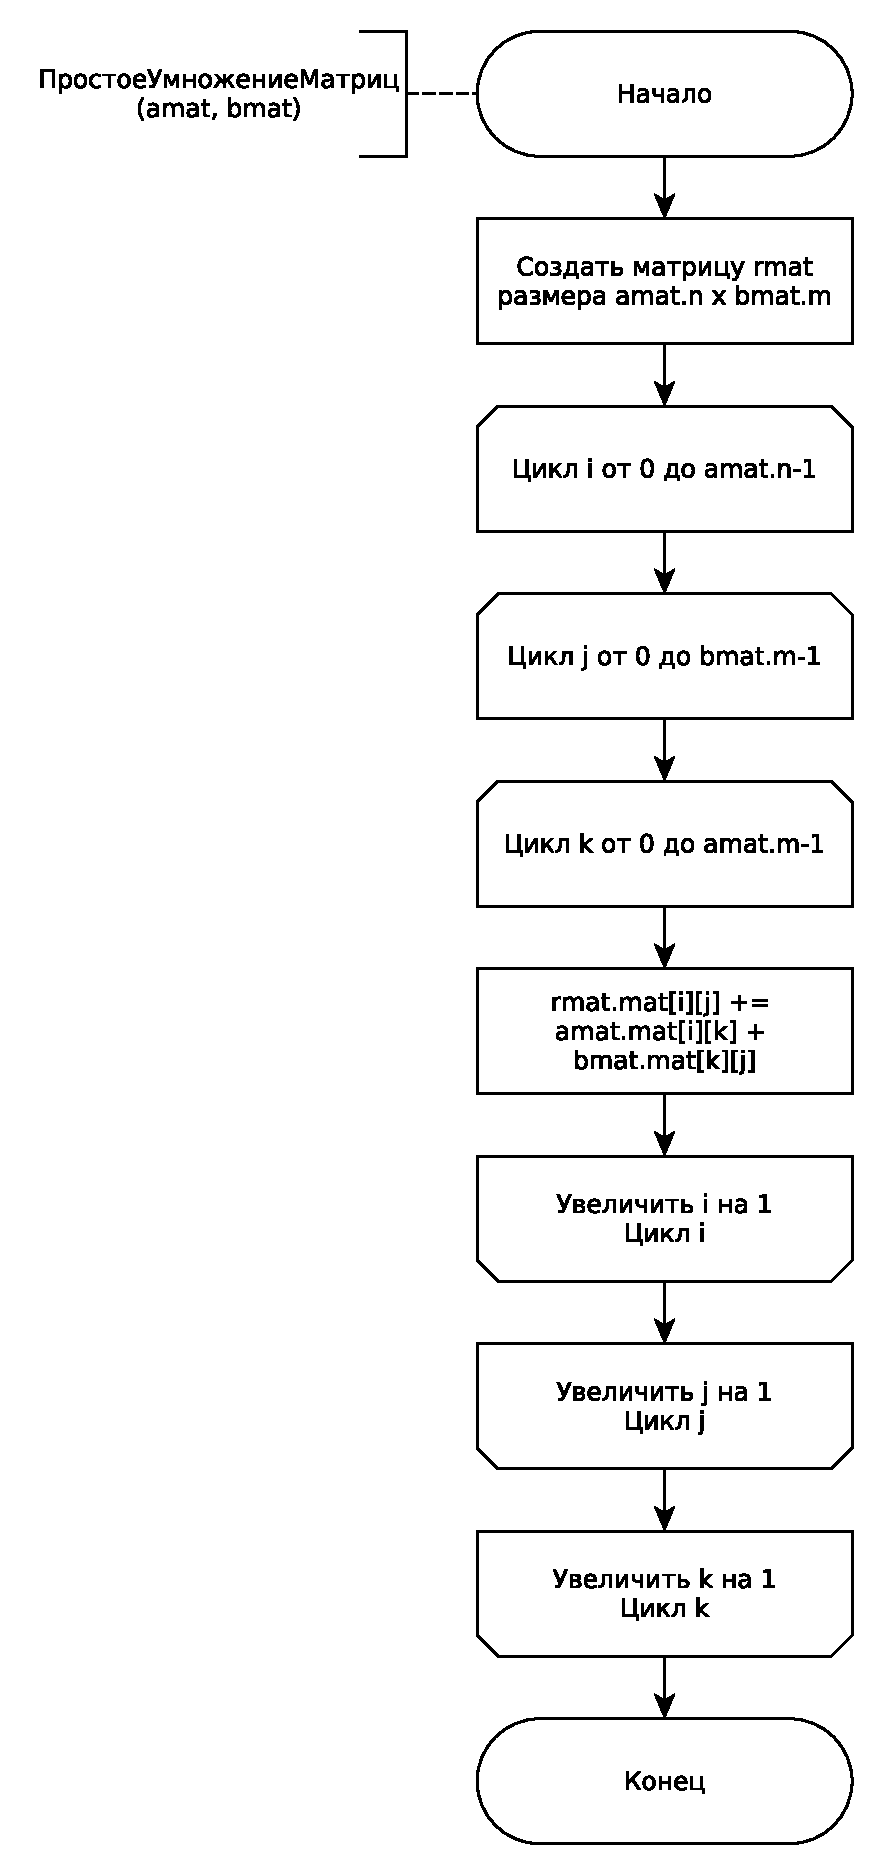
\includegraphics[width=0.65\linewidth]{assets/mtx-alg.pdf}
	\caption{Схема классического алгоритма умножения матриц}
	\label{fig:alg}
\end{figure}
% УБрать MH MV
\begin{figure}[ht!]
	\centering
	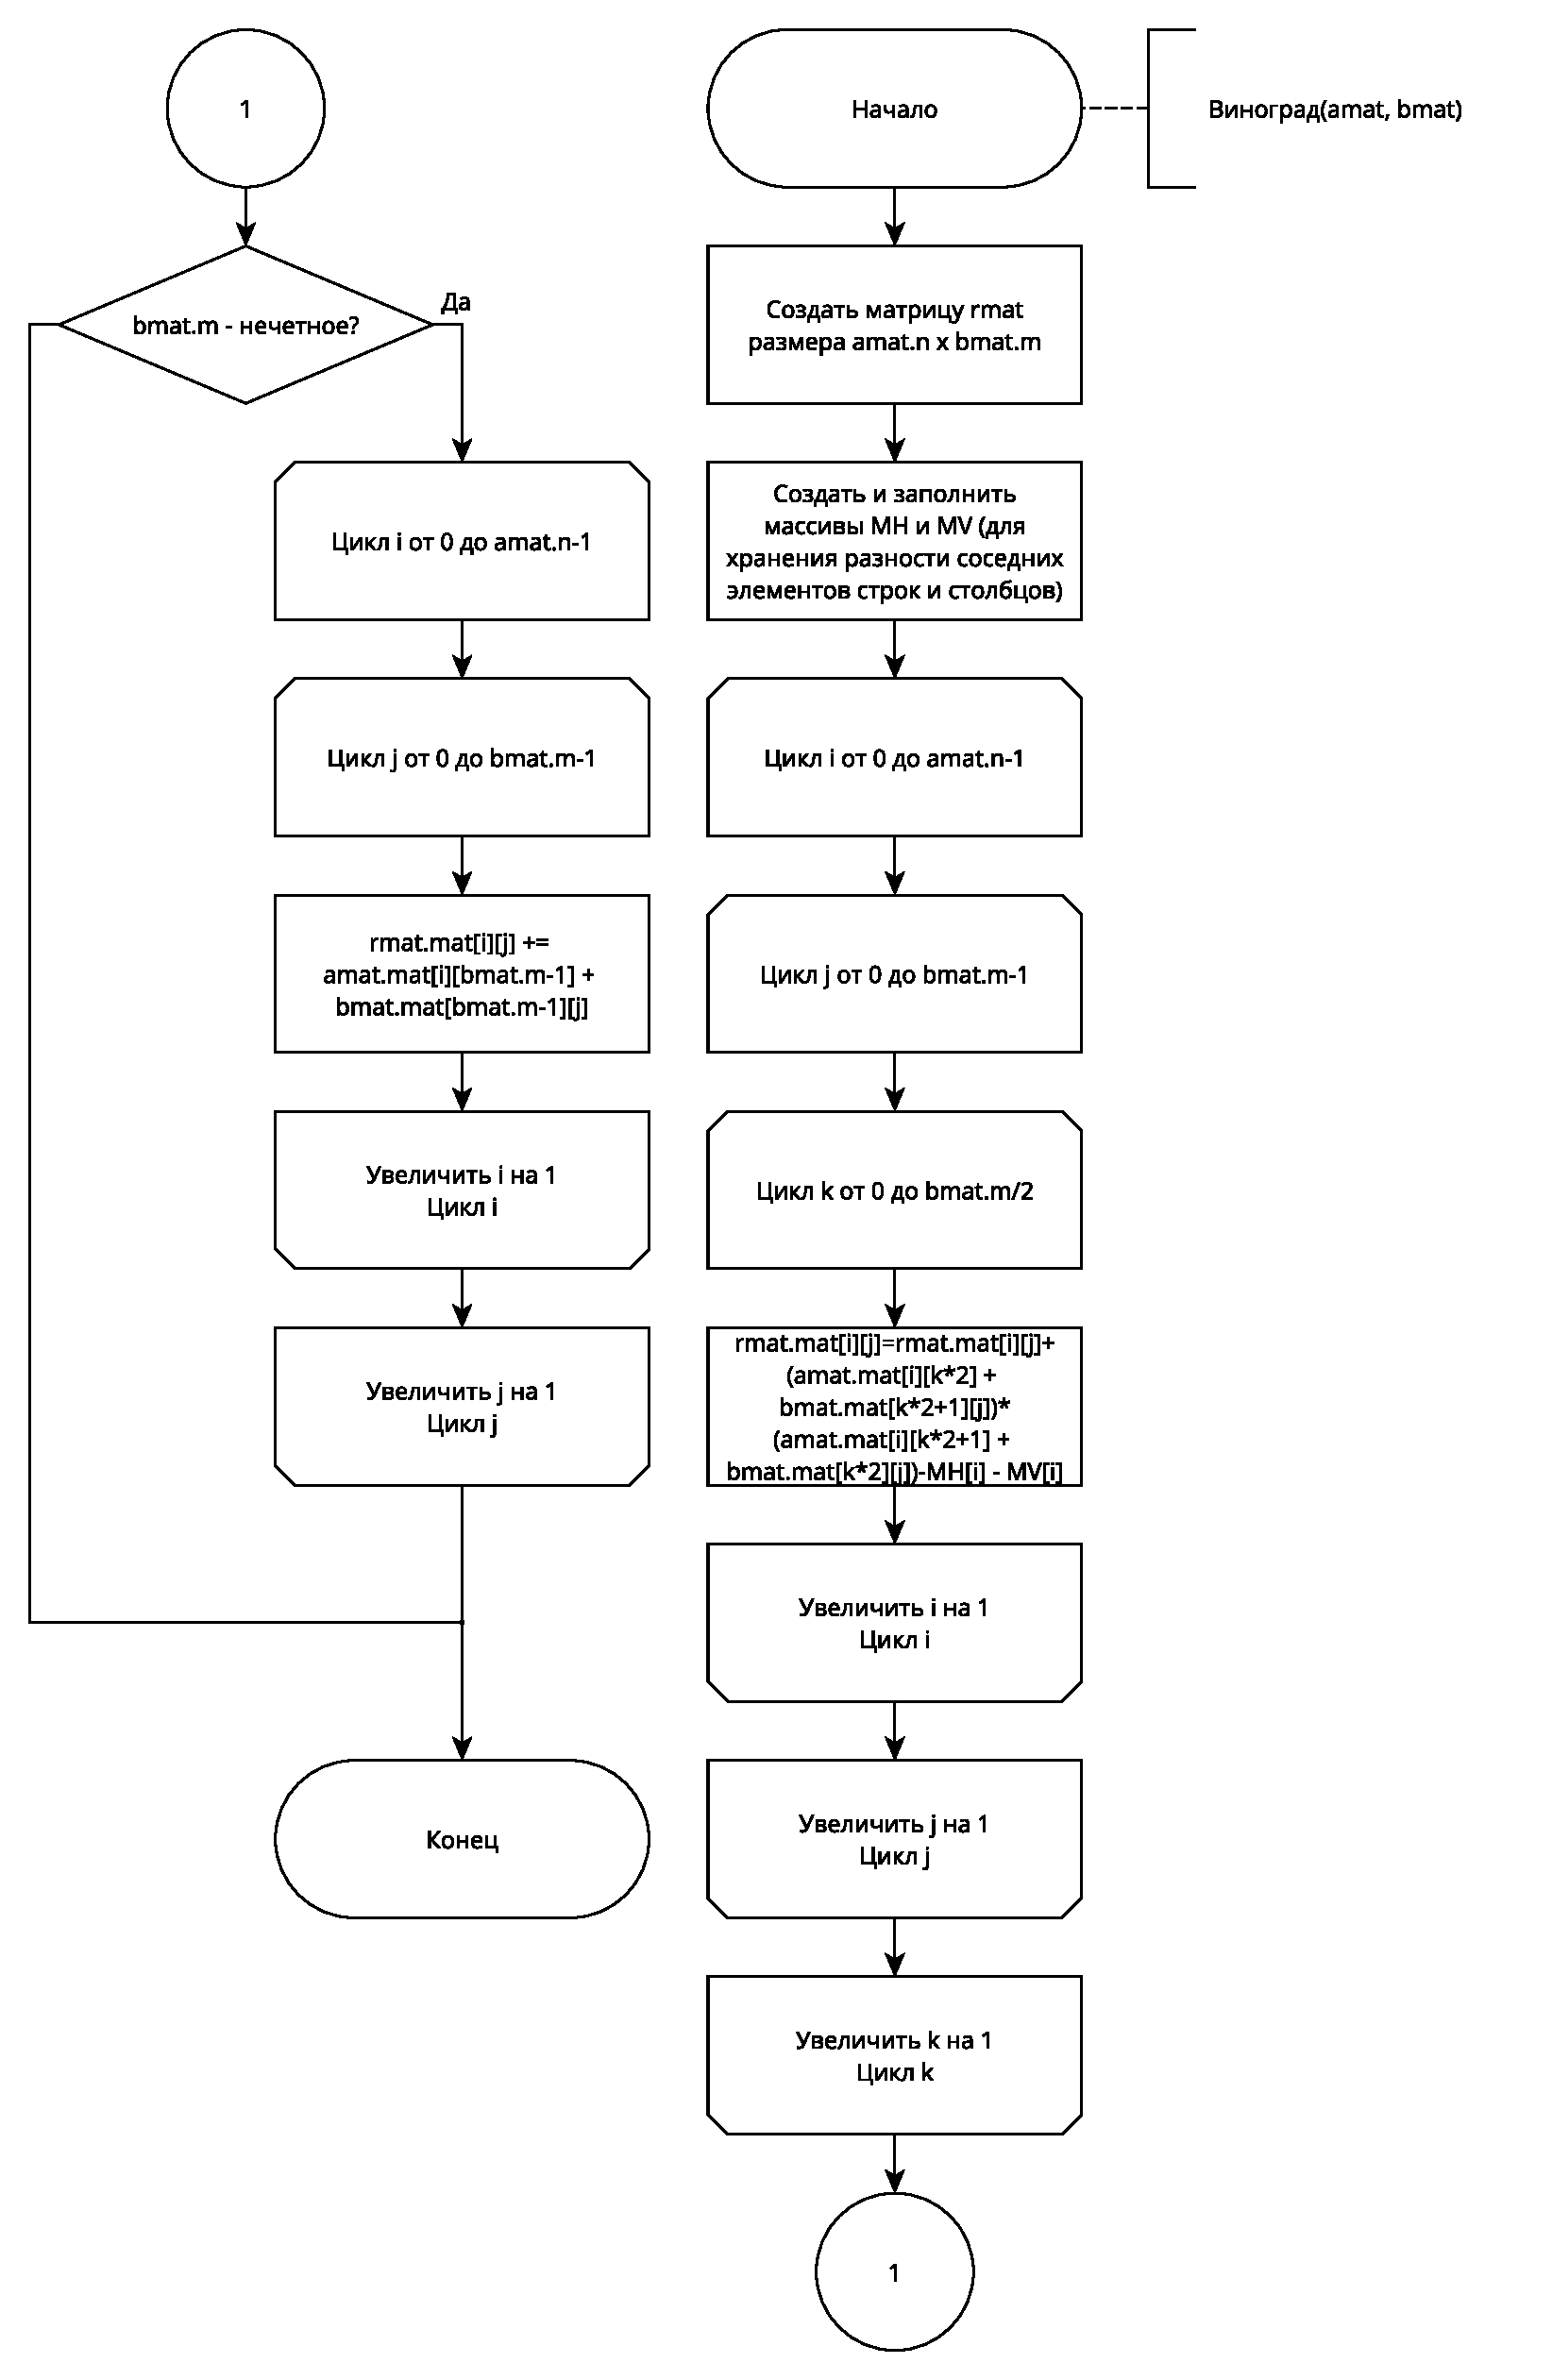
\includegraphics[width=0.95\linewidth]{assets/mtx-win1.pdf}
	\caption{Схема алгоритма умножения матриц Винограда}
	\label{fig:win-1}
\end{figure}
% Переставить MH MV, счетчики циклов поменять
\begin{figure}[ht!]
	\centering
	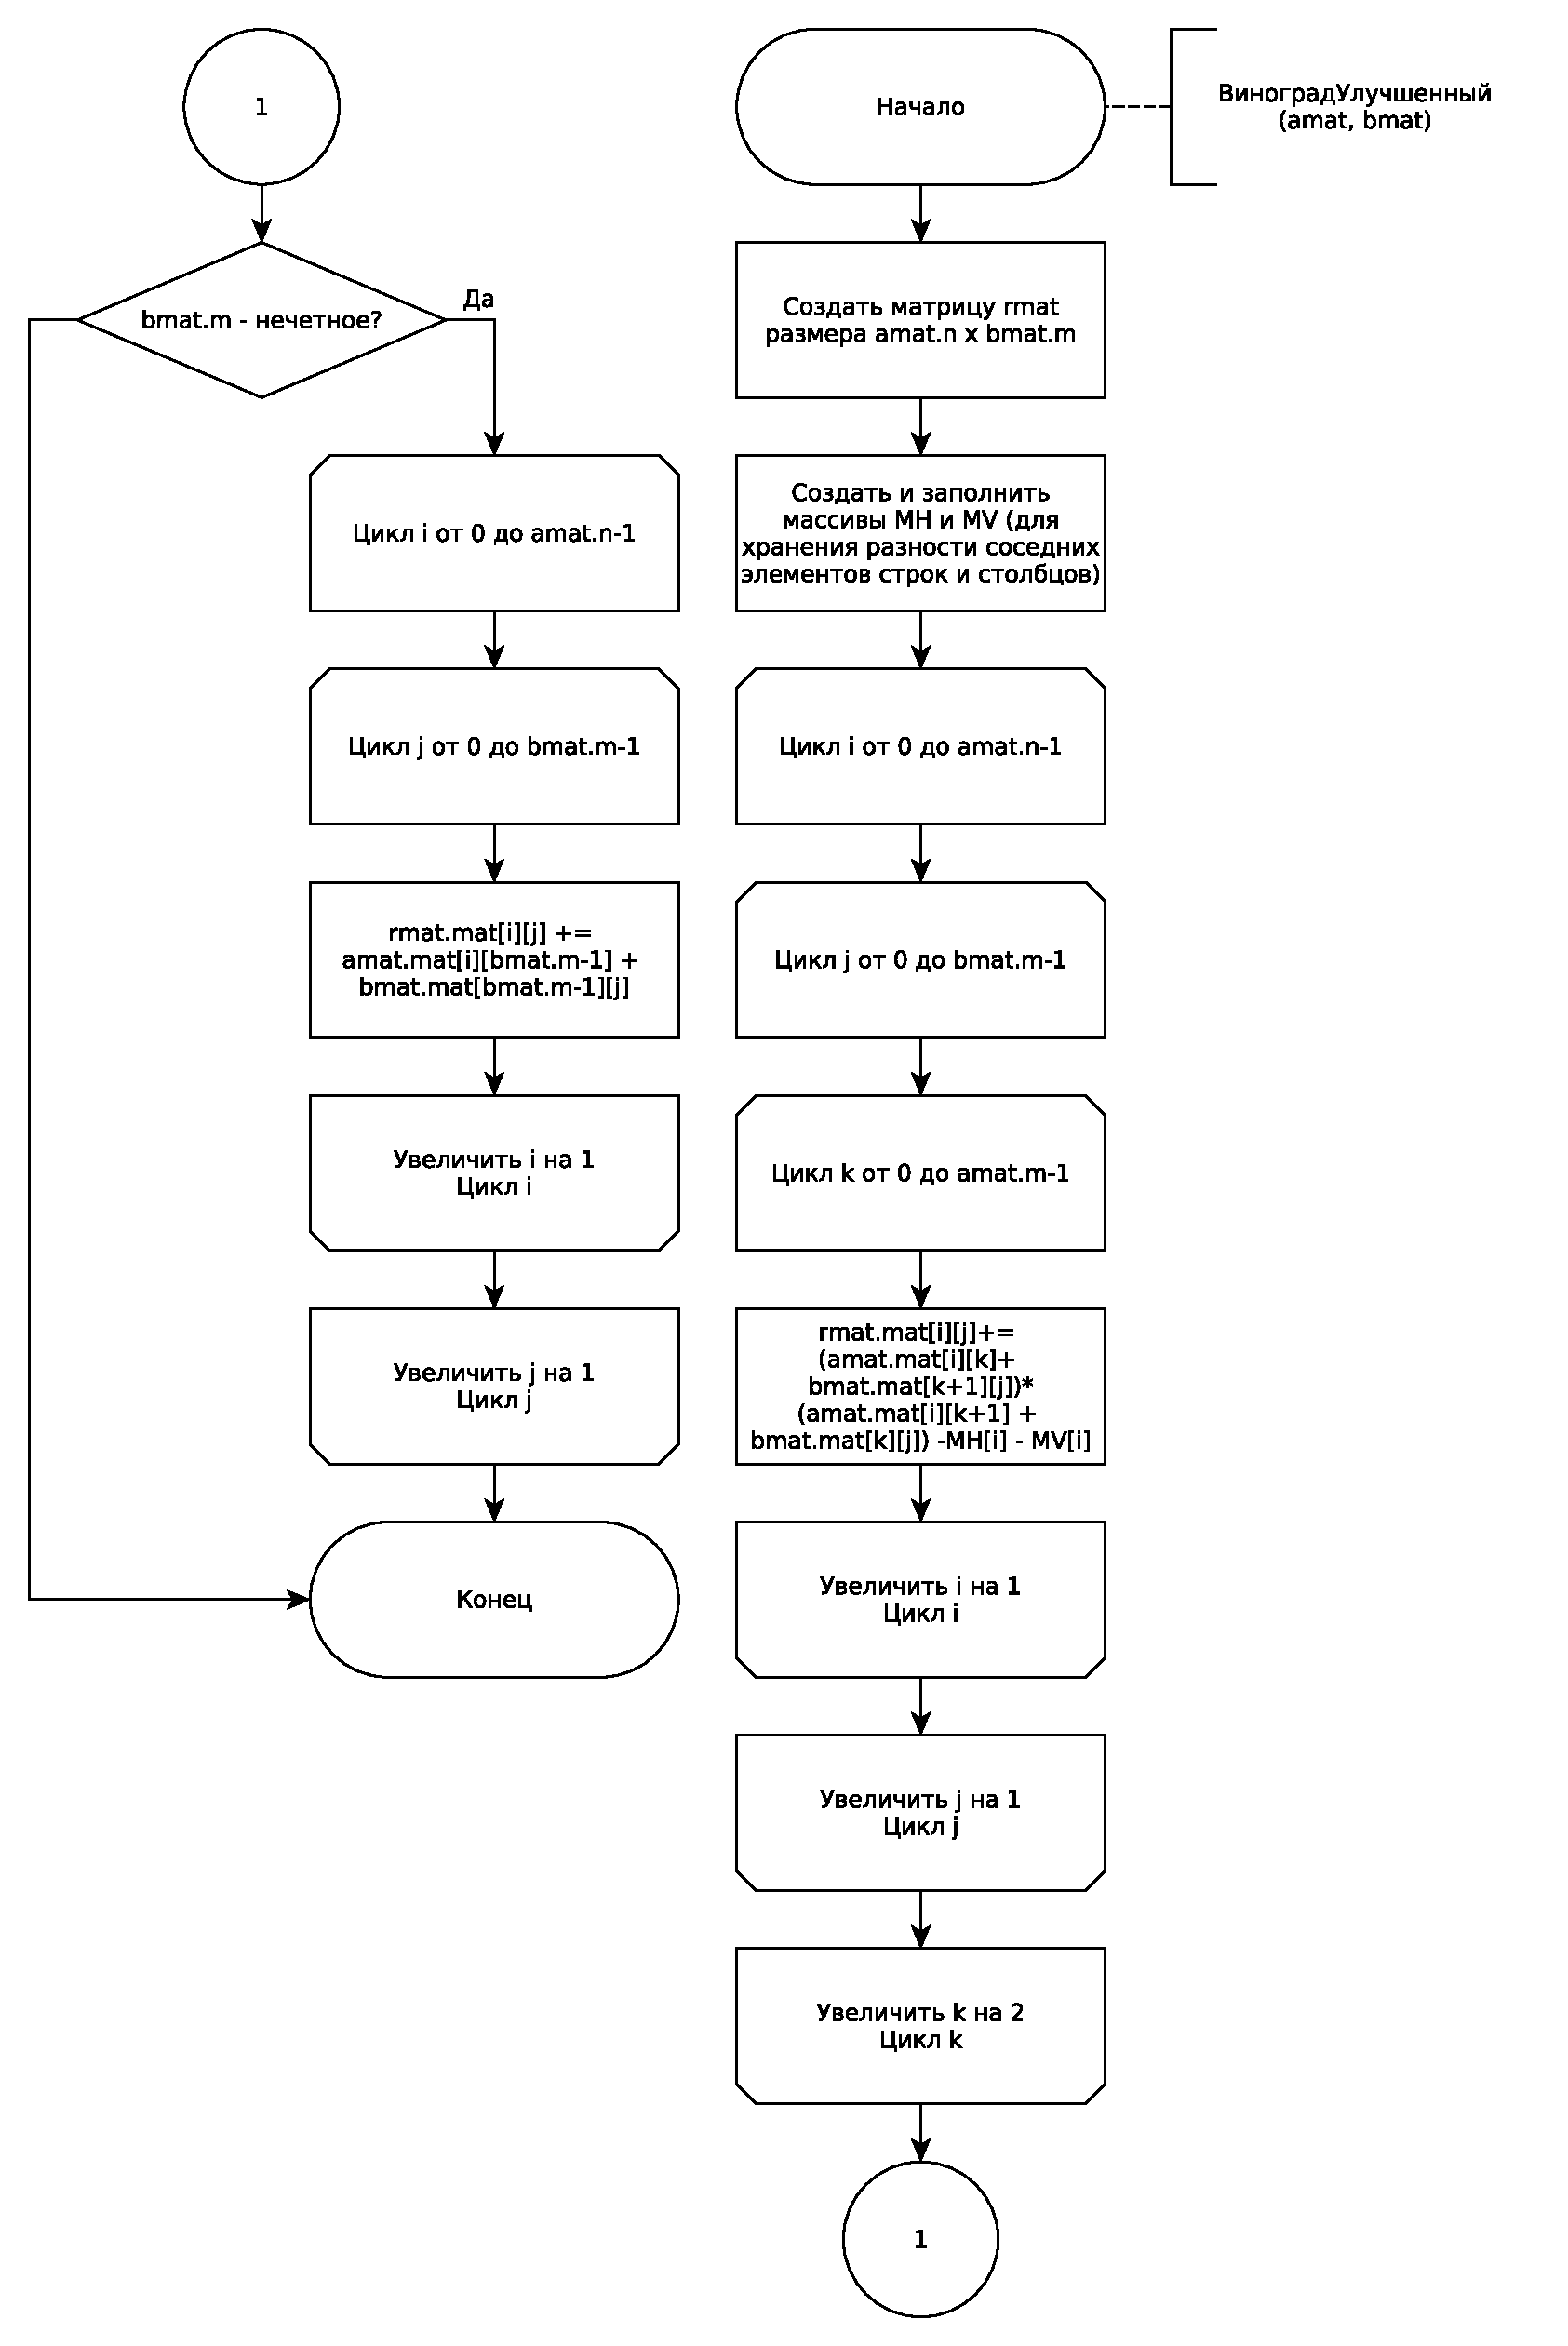
\includegraphics[width=0.75\linewidth]{assets/mtx-win2.pdf}
	\caption{Схема оптимизированного алгоритма умножения матриц Винограда}
	\label{fig:win-2}
\end{figure}

\newpage
\section*{Вывод}
Алгоритмы были проанализированы с точки зрения временных затрат. Было выявлено, что оптимизированный алгоритм  Винограда имеет трудоемкость в 1.5 раза меньше, чем классический алгоритм Винограда.


Были построены схемы алгоритмов. Были выделены способы оптимизации алгоритма Винограда. Было получено достаточно теоретических сведений для разработки ПО, решающего поставленную задачу.